% =====================================================================
%  Final Dissertation — Emergent Social Behaviour & Dilemmas in MARL
%  Ahmed Wael Elsisi (214647) — The British University in Egypt
%  Compiles with pdflatex, xelatex, or tectonic.
% =====================================================================
\documentclass[12pt,a4paper]{report}

\usepackage[utf8]{inputenc}
\usepackage[T1]{fontenc}
\usepackage[a4paper,margin=1in]{geometry}
\usepackage{graphicx}
\usepackage{amsmath,amssymb}
\usepackage{booktabs}
\usepackage{siunitx}
\usepackage{caption}
\usepackage{subcaption}
\usepackage{float}
\usepackage{xcolor}
\usepackage{enumitem}
\usepackage[numbers,sort&compress]{natbib}
\usepackage[hidelinks]{hyperref}

\graphicspath{{figures/}}
\captionsetup{font=small,labelfont=bf}
\setlength{\parskip}{0.4em}

% Convenience macros
\newcommand{\mappo}{MAPPO}
\newcommand{\ippo}{IPPO}
\newcommand{\grid}[1]{$#1\times#1$}

\begin{document}

% ----------------------------- TITLE PAGE -----------------------------
\begin{titlepage}
\centering
\vspace*{1.5cm}
{\LARGE\bfseries Emergent Social Behaviour \& Dilemmas in\\[0.3em]
Multi-Agent Reinforcement Learning\par}
\vspace{1.0cm}
{\large By\par}
\vspace{0.3cm}
{\large Ahmed Wael Elsisi --- 214647\par}
\vspace{1.5cm}
{\normalsize A Dissertation submitted to the Faculty of Engineering, The British
University in Egypt, in Partial Fulfilment of the requirements for the
bachelor's degree in Electrical Engineering\par}
\vspace{1.5cm}
{\large Supervisor: Dr.\ Randa Mohamed\par}
\vspace{2.0cm}
{\normalsize June 2026\par}
{\normalsize Electrical Engineering Department\par}
{\normalsize Computer Engineering Programme\par}
\vfill
\end{titlepage}

\pagenumbering{roman}
\chapter*{Abstract}
\addcontentsline{toc}{chapter}{Abstract}

Multi-agent reinforcement learning (MARL) increasingly powers autonomous systems,
from traffic control to distributed energy grids, yet a fundamental question
remains open: when does an explicit \emph{coordination mechanism} actually help, and
when do independent learners suffice? This dissertation answers that question on a
controlled, inherently cooperative benchmark --- traffic signal control on a
$2\times2$ grid of four intersections in SUMO, integrated with Ray RLlib.

A Multi-Agent Proximal Policy Optimization (MAPPO) controller, with a centralized
critic and a neighbour-coupled reward, was implemented and trained to stable
convergence. Under a \emph{fair, matched-clearance} evaluation --- in which every
controller pays the same realistic safety clearance --- the learned controller
decisively outperforms both the fixed-time and max-pressure heuristics; a
methodological finding of this work is that the heuristics' apparent strength was an
artefact of an unfair zero-clearance evaluation. The project's MAPPO was further
confirmed to match the canonical published recipe of Yu~et~al.\ (2021), establishing
it as a faithful, competitive implementation rather than a weak strawman.

The central result is a surprise. Compared against Independent PPO (IPPO) --- a fully
decentralized comparator differing only in its decentralized critic and purely local
reward --- MAPPO proves \emph{statistically indistinguishable} on every
traffic-performance metric across five seeds; the only reliable difference is that
the cooperative controller performs slightly more phase switches, with no
performance benefit. On a $2\times2$ network the \emph{coordination value}
(MAPPO~$-$~IPPO) is therefore approximately zero. The interpretation is not that
coordination is worthless but that the network is small enough that incentives are
already locally aligned, so independent learners recover coordinated behaviour
implicitly. This locates precisely where explicit coordination should begin to pay
off --- at larger network scales --- and motivates the future work of scaling to a
$5\times5$ grid and of extending the study to genuine social dilemmas, both placed
beyond this submission by compute constraints. The contribution is thus a careful
negative result together with a sharpened hypothesis: the value of cooperation in
MARL is not a fixed property of an algorithm but a function of scale.


\tableofcontents
\listoffigures
\listoftables
\clearpage
\pagenumbering{arabic}

\chapter{Introduction}
\label{ch:intro}

\section{Problem Statement}
Multi-agent systems --- where several autonomous agents interact to achieve goals
individually or collectively --- underpin a growing share of modern technology.
Autonomous vehicles share roads, distributed sensors coordinate surveillance, and
energy grids balance supply across many producers. Unlike traditional control
systems with a single centralized decision maker, these settings contain
independent agents that must learn to coexist, coordinate, or compete. The
difficulty is not merely making each agent individually competent; it is
understanding what emerges when many \emph{learning} agents interact.

Reinforcement learning (RL) is a paradigm in which an agent learns to act by
interacting with an environment and receiving reward feedback. Extending RL to
many simultaneously learning agents --- Multi-Agent Reinforcement Learning
(MARL) --- changes the problem fundamentally. Each agent treats the others as part
of its environment, yet those ``parts'' are themselves learning and changing:
today's optimal response can fail tomorrow once the others adapt. This
\emph{non-stationarity} breaks the assumptions that make single-agent RL
convergent and stable.

Crucially, the \emph{relationship} between agents varies. Sometimes cooperation
benefits everyone; at other times genuine conflict arises, and an agent can
exploit a shared resource for private gain while pushing the cost onto the
collective. Knowing \emph{when} cooperation emerges versus \emph{when}
exploitation dominates is central to deploying autonomous agents responsibly.

This dissertation studies cooperation in MARL using \emph{traffic signal control}
as a representative, inherently cooperative case study. Each intersection is an
agent; because network effects mean that gridlock hurts everyone (including the
intersection that caused it), traffic sits at the \emph{pure-coordination} end of
the cooperation spectrum and is an ideal testbed for isolating the value of
explicit coordination mechanisms.

\section{Research Gap}
Despite rapid progress, several questions remain underexplored:

\begin{itemize}[leftmargin=1.4em]
  \item \textbf{The middle of the spectrum.} Most work targets either purely
  cooperative settings or purely competitive games (chess, poker). The continuum
  between them --- where coordination and competition coexist --- receives less
  systematic study.
  \item \textbf{Reward structure.} While reward shaping is known to matter,
  controlled comparisons of \emph{individual} versus \emph{shared} objectives
  across standardized environments are rare.
  \item \textbf{Fairness.} Algorithms typically optimize total system performance
  without examining how benefits distribute across agents.
  \item \textbf{Scalability of coordination.} How the \emph{value} of a
  coordination mechanism changes as a system grows --- from a handful of agents to
  large networks --- has not been systematically characterized.
\end{itemize}

This work contributes to the first and fourth gaps directly. It asks a deceptively
simple question on a controlled traffic benchmark: \emph{does an explicitly
cooperative algorithm (MAPPO, with a centralized critic) actually outperform a set
of independent learners (IPPO) when the two are matched in every other respect?}
The answer --- and the reason behind it --- forms the spine of this dissertation.

\chapter{Background and Literature Review}
\label{ch:background}

\section{Reinforcement Learning}
Reinforcement learning provides a mathematical framework for an agent learning
optimal behaviour through interaction. Its foundation is the Markov Decision
Process (MDP): a set of \emph{states} describing the environment, \emph{actions}
the agent may take, \emph{transition dynamics} mapping state--action pairs to next
states, and a \emph{reward} signal. The agent seeks a \emph{policy} --- a mapping
from states to actions --- that maximizes the expected cumulative discounted
return. This is captured by the Bellman equation~\cite{sutton2018}, which expresses
the value of a state as the immediate reward plus the discounted value of its
successor, enabling algorithms to \emph{bootstrap} value estimates from one another.
Classical methods such as Q-learning iteratively estimate the optimal action-value
function after each interaction, addressing the \emph{credit assignment} problem of
attributing outcomes to past actions.

\section{Deep Reinforcement Learning}
Tabular methods store a value for every state--action pair and become infeasible in
large or continuous state spaces. Deep Reinforcement Learning (DRL) replaces the
table with a neural-network function approximator. The Deep Q-Network (DQN)
pioneered this with \emph{experience replay} (sampling past transitions to break
temporal correlation) and \emph{target networks} (stabilizing the bootstrap target).

Whereas DQN is value-based, \emph{policy-gradient} methods directly optimize the
policy by ascending the expected return. Proximal Policy Optimization
(PPO)~\cite{schulman2017ppo} has become the standard modern choice: it constrains
how far the policy may move in a single update through a clipped surrogate
objective, preventing the destructive updates that destabilized earlier methods
while remaining simple and sample-efficient. Generalized Advantage Estimation
(GAE)~\cite{schulman2016gae} complements PPO by trading off bias and variance in
the advantage estimate through exponentially weighted temporal-difference errors;
it is now standard in policy-gradient implementations.

\section{Multi-Agent Reinforcement Learning}

\subsection{Fundamental Challenges}
Extending RL to multiple agents introduces complications absent in the
single-agent case. \textbf{Non-stationarity} is the central one: each agent
perceives the others as part of its environment, but those components evolve as the
others learn, violating the stationary-transition (Markov) assumption and voiding
single-agent convergence guarantees. \textbf{Credit assignment} also becomes
harder: when a team shares a reward, attributing it to individual actions is
difficult, and the joint action space grows exponentially (e.g.\ four agents with
four actions yield $4^4 = 256$ combinations). \textbf{Scalability} therefore
demands decomposing the global problem into local subproblems each agent can solve
from its own observation.

\subsection{Algorithmic Approaches}
\textbf{Independent Q-Learning (IQL)}~\cite{tan1993iql} is the simplest approach:
each agent learns its own value function, treating the others as environment and
ignoring non-stationarity entirely. It is simple and scalable, often works in
practice when mutual influence is limited, but lacks convergence guarantees and
struggles with cooperative credit assignment. Its policy-gradient analogue,
\textbf{Independent PPO (IPPO)}, applies PPO independently per agent and is the
``fully independent learners'' baseline used throughout this work.

\textbf{Value-decomposition} methods address credit assignment by learning how
individual values combine into a team value. \textbf{QMIX}~\cite{rashid2018qmix}
represents the joint action-value as a \emph{monotonic} mixture of individual
values, guaranteeing that improving an individual's value improves the team's,
while permitting decentralized execution.

These advances rest on the \textbf{Centralized Training with Decentralized
Execution (CTDE)} paradigm. Under CTDE, training may use privileged global
information (all agents' observations and actions) to stabilize learning and tame
non-stationarity, but the deployed policies act only on local observations,
preserving scalability and requiring no inter-agent communication at run time. A
useful analogy is a sports team: in practice a coach observes all players and
teaches coordination; in the match, players act independently on their local view,
applying what they learned.

\textbf{MADDPG}~\cite{lowe2017maddpg} pioneered CTDE for actor--critic methods with
centralized critics that see all agents' observations and actions during training
and decentralized actors at execution. \textbf{MAPPO}~\cite{yu2021mappo} combines
this centralized-critic architecture with PPO's robust optimization: a shared
centralized value function consumes all agents' observations during training, each
agent keeps its own decentralized policy, PPO clipping prevents destructive
updates, and GAE stabilizes advantages. MAPPO is reported to match or beat more
specialized cooperative algorithms across standard benchmarks, which is precisely
why it is the natural ``sophisticated cooperative method'' to test here.

Table~\ref{tab:algos} summarizes these algorithms.

\begin{table}[H]
\centering
\caption{Comparison of representative MARL algorithms.}
\label{tab:algos}
\small
\begin{tabular}{@{}llll@{}}
\toprule
\textbf{Algorithm} & \textbf{Training} & \textbf{Execution} & \textbf{Key characteristics} \\
\midrule
IQL / IPPO & Independent       & Decentralized & Simple, scalable; treats others as \\
           &                   &               & environment; unstable under non-stationarity \\[0.3em]
QMIX       & Centralized mixer & Decentralized & Monotonic value factorisation; \\
           &                   &               & cooperative settings only \\[0.3em]
MADDPG     & Centralized critic& Decentralized & Actor--critic CTDE; continuous actions; \\
           &                   &               & less stable, limited scalability \\[0.3em]
MAPPO      & Centralized critic& Decentralized & PPO-based; stable; strong coordination \\
           &                   &               & and scalability \\
\bottomrule
\end{tabular}
\end{table}

\section{Social Dilemmas in Multi-Agent Systems}
Social dilemmas describe situations where individually rational behaviour yields a
collectively poor outcome. The \emph{Prisoner's Dilemma} is canonical: both agents
benefit from mutual cooperation, yet each maximizes its own payoff by defecting
regardless of the other, so rational self-interest drives both to a worse outcome.
The \emph{Tragedy of the Commons} extends this to shared resources: each user
benefits from exploitation while the cost is distributed, creating pressure toward
overexploitation that destroys the resource for all. \emph{Sequential social
dilemmas}~\cite{leibo2017ssd} embed such incentives in grid-world environments over
many timesteps; the ``Harvest'' commons, where agents collect slowly regrowing
apples and over-harvesting permanently depletes a region, is a standard example.
Social dilemmas sit at the \emph{opposite} end of the spectrum from traffic and are
discussed as future work (Chapter~\ref{ch:futurework}).

\section{MARL for Traffic Signal Control}
Traffic signal control is naturally modelled as MARL: each traffic light is an
agent that observes local traffic state, selects a signal phase, and is rewarded
for traffic efficiency. Because intersections interact through traffic flow, agents
must learn policies that are good for the whole network, not just locally.
Traditional fixed-time and actuated controllers require manual tuning and cope
poorly with non-recurring congestion; RL promises adaptive controllers that learn
from experience. Early single-intersection deep-RL controllers improved on
classical methods but missed network effects, where a locally optimal decision
creates downstream problems.

\textbf{CoLight}~\cite{wei2019colight} addressed this by giving each agent
information about adjacent intersections and sharing network parameters across
agents, inducing coordinated behaviour despite decentralized execution. A
particularly effective family is \emph{pressure-based} control, which minimizes the
imbalance between incoming and outgoing vehicle counts per movement and connects to
max-pressure control from transportation theory. A large-scale
comparison~\cite{chu2020largescale} found that sharing neighbour information
significantly improves network performance \emph{but only with careful reward
design}: naive individual rewards, where each intersection minimizes only its own
delay, can harm overall throughput, whereas shared rewards help but demand careful
algorithm design to scale.

A central observation motivates this dissertation: from a system designer's
viewpoint traffic is \emph{fundamentally cooperative}. Network effects align
incentives --- gridlock hurts everyone --- which makes traffic an excellent,
controlled environment for asking whether an explicit coordination mechanism is
actually \emph{necessary}, or whether independent learners can recover the same
behaviour on their own.

\chapter{Objectives}
\label{ch:objectives}

The overarching aim of this research is to study emergent social behaviour,
cooperation, and the value of coordination in Multi-Agent Reinforcement Learning,
using traffic signal control as a controlled, inherently cooperative case study.
The realized objectives of this dissertation are:

\begin{enumerate}[leftmargin=1.6em]
  \item \textbf{Establish a strong cooperative baseline.} Implement and train a
  MAPPO traffic-signal controller on a \grid{2} grid and demonstrate stable
  convergence, then validate it against the standard heuristic controllers
  (fixed-time and max-pressure) under a \emph{fair} evaluation protocol.

  \item \textbf{Confirm implementation fidelity.} Compare the project's MAPPO
  configuration against the canonical published recipe of
  Yu~et~al.~\cite{yu2021mappo}, to establish that the cooperative agent is a faithful,
  competitive implementation and not a weakened strawman.

  \item \textbf{Quantify the value of coordination.} Implement Independent PPO
  (IPPO) as a fully decentralized comparator that differs from MAPPO only in its
  two defining design choices --- a decentralized critic and a purely local reward
  --- and measure the \emph{coordination value}, defined as the performance
  difference $\text{MAPPO} - \text{IPPO}$.

  \item \textbf{Characterize and interpret the result.} Analyze \emph{why} the
  measured coordination value takes the value it does at this network scale, and
  connect the finding to the broader question of how coordination mechanisms scale
  with network complexity.
\end{enumerate}

Two further aims --- characterizing the efficiency--equity trade-off and contrasting
coordination against genuine social dilemmas --- motivate the future work outlined in
Chapter~\ref{ch:futurework}, where network scale-up and a social-dilemma
environment are identified as the natural next steps that compute constraints
placed beyond the scope of this submission.

\chapter{Methodology}
\label{ch:methodology}

This chapter describes the environment, the agent design shared by all learned
controllers, the two algorithms under comparison (MAPPO and IPPO), the published
paper-baseline used as a fidelity check, and --- importantly --- the \emph{fair}
evaluation protocol under which all controllers are compared.

\section{Environment}
The environment is a \grid{2} grid network of four signalized intersections
(\texttt{J1}--\texttt{J4}), each controlled by one agent, simulated in SUMO
(Simulation of Urban MObility) and driven through the TraCI interface, integrated
with the Ray RLlib framework. Roads between intersections are \SI{150}{\metre} and
entry/exit roads \SI{100}{\metre}; each road has three lanes with strict
directional assignment (lane~0 right turns, lane~1 straight, lane~2 left turns).
Lane-area detectors span each lane for full observability of positions, speeds and
waiting times. An episode lasts \SI{3600}{\second} of simulation with a
\SI{5}{\second} action interval, giving up to 720 decision points per agent.
Demand follows a realistic profile: light traffic ($0$--\SI{600}{\second}), a rush
hour (\SI{600}{}--\SI{2400}{\second}), then light traffic again.

\section{Observation, Action and Reward}

\subsection{Observation space (70 dimensions per agent)}
Each agent observes a 70-dimensional vector: \textbf{28 local} features ---
per-movement queue lengths (12), one-hot current phase direction (2), normalized
elapsed phase time (1), movement pressures, i.e.\ incoming minus outgoing counts
(6), pressure derivatives (6), and a binary min-green flag (1) --- and \textbf{42
neighbour} features from the two adjacent intersections (21 each), carrying shared
queues, neighbour phase, combined pressures, and directional incoming/outgoing
metrics, spatially discounted with $\gamma_s = 0.9$ to weight nearer intersections
more heavily.

\subsection{Action space}
The action space is discrete with four green phases following traffic-engineering
standards: north--south through/right, north--south left, east--west
through/right, and east--west left. Right turns are permissive in all phases.

\subsection{Reward function}
The reward combines five weighted components (configuration~v2):
\begin{equation}
r_t = -1.0\,W_t \;-\; 0.25\,Q_t \;+\; 0.1\,T_t \;-\; 0.4\,P_t \;-\; 0.4\,N_t,
\end{equation}
where $W_t$ is cumulative waiting time (the primary objective), $Q_t$ the queue
length, $T_t$ the network throughput (a shared term), $P_t$ the local pressure
(incoming minus outgoing queue imbalance), and $N_t$ the spatially discounted
\emph{neighbour} pressure ($\gamma_s = 0.9$) that couples each agent to its
neighbours. The reward is clipped to $[-3.0, 1.0]$. The neighbour term $N_t$ is the
sole explicit multi-agent coupling in the reward and is the lever that
distinguishes MAPPO from IPPO (Section~\ref{sec:algos}).

\section{Network Architectures}
All learned agents share a single policy (parameter sharing across the four
homogeneous intersections). The \textbf{actor} is decentralized: it maps the
agent's 70-dimensional local observation through two hidden layers of 256 units
with $\tanh$ activations to four action logits. The MAPPO \textbf{critic} is
\emph{centralized}: it consumes the 280-dimensional global state (the four agents'
70-dimensional observations concatenated) through hidden layers of 512, 256 and 128
units with ReLU activations to a single value. Orthogonal initialization and a
running observation normalizer (\texttt{MeanStdFilter}) are used throughout.

\section{Algorithms Under Comparison}
\label{sec:algos}
The comparison is designed so that MAPPO and IPPO differ \emph{only} in the two
design choices that define ``cooperative MARL'' versus ``independent learners'';
every other hyperparameter and the actor architecture are identical.

\begin{itemize}[leftmargin=1.4em]
  \item \textbf{MAPPO (cooperative).} Centralized critic over the 280-dimensional
  global state; the neighbour-pressure reward term $N_t$ is active. This is the
  ``full cooperative package'': CTDE training plus an explicitly coordination-aware
  reward.
  \item \textbf{IPPO (independent).} Decentralized critic that sees only the
  agent's own 70-dimensional observation; the neighbour-pressure weight is set to
  zero so each agent optimizes a purely local objective. Parameter sharing is
  retained. This is the ``fully independent learners'' package.
\end{itemize}

\noindent The shared hyperparameters (configuration~v2) are listed in
Table~\ref{tab:hparams}.

\begin{table}[H]
\centering
\caption{Shared training hyperparameters (MAPPO~v2 and IPPO).}
\label{tab:hparams}
\small
\begin{tabular}{@{}lll@{}}
\toprule
\textbf{Hyperparameter} & \textbf{Value} & \textbf{Note} \\
\midrule
Learning rate            & $5\times10^{-4}$ & \\
Discount factor $\gamma$ & $0.99$           & long-horizon optimization \\
GAE $\lambda$            & $0.95$           & bias--variance trade-off \\
PPO clip $\epsilon$      & $0.2$            & \\
Value clip               & $10.0$           & \\
Gradient clip            & $1.0$            & \\
Entropy coefficient      & $0.02$           & exploration \\
Value-loss coefficient   & $1.0$            & \\
SGD iterations/update    & $15$             & \\
Minibatch / train batch  & $32768 / 32768$  & full-batch update \\
Rollout workers          & $3$              & \\
Rollout fragment         & $200$            & complete-episode batching \\
Training iterations      & $200$            & \\
Observation filter       & MeanStdFilter    & running mean/std \\
\bottomrule
\end{tabular}
\end{table}

\subsection{Paper-baseline (fidelity check)}
To confirm that the project's MAPPO is not an under-powered strawman, it is also
compared against the canonical recipe of Yu~et~al.~\cite{yu2021mappo} (their adopted
MLP preset): actor and critic both two hidden layers of 512 units with ReLU, actor
learning rate $7\times10^{-4}$, 15 SGD iterations per update, a single full-batch
minibatch, clip $0.2$, entropy coefficient $0.015$, and gradient clipping at
$10.0$. All three controllers (MAPPO~v2, IPPO, paper-baseline) are trained for 200
iterations under identical environment dynamics.

\section{Baseline Controllers}
Two standard heuristics provide reference points. The \textbf{fixed-time}
controller cycles phases on a fixed schedule. The \textbf{max-pressure} controller
selects, at each decision, the phase that maximizes the relief of pressure
(incoming minus outgoing queue imbalance), subject to a minimum green time.

\section{Fair Evaluation Protocol}
\label{sec:fairproto}
A controlled comparison requires that every controller pay the same real-world
operating costs. Two points are essential.

\paragraph{Matched safety clearance.} The learned agents operate with a
\SI{3}{\second} all-red clearance on every phase change (\texttt{min\_red}~$=3$), a
realistic safety constraint they were \emph{trained} under. The heuristic
controllers, by default, switched phases instantaneously (zero clearance), which
silently advantaged them. All controllers are therefore evaluated with the
\emph{same} \SI{3}{\second} clearance; the consequences of ignoring this are
quantified in Chapter~\ref{ch:results}.

\paragraph{Faithful policy evaluation.} With RLlib's connector-enabled inference,
the running observation normalizer is not applied automatically at evaluation; it is
applied manually so the deterministic policy receives the same input distribution it
saw in training (omitting it collapses the policy). Neighbour edge-connectivity
metadata is likewise forwarded into the evaluation environment so the full
70-dimensional observation is reconstructed. Each controller is evaluated over five
seeds ($42$--$46$); per-metric means, standard deviations, and Welch's $t$-tests are
reported in Chapter~\ref{ch:results}.

\chapter{Results and Analysis}
\label{ch:results}

This chapter presents the empirical findings in the order that tells the story:
the cooperative controller is first shown to train well and to beat the heuristic
baselines under a fair evaluation; it is then confirmed to be a faithful
implementation of the published method; and finally it is compared head-to-head
against independent learners, with a result that inverts the natural expectation.

\section{Training Convergence}
The MAPPO controller (configuration~v2) trains stably to convergence over 200
iterations. The mean episode reward improves from $-2756.5$ at initialization to a
converged last-ten-iteration mean of $-49.76 \pm 0.41$
(Figure~\ref{fig:trainreward}). The centralized critic is accurate, reaching a
value-function explained variance of $0.907$, and policy updates remain
conservative, with an average KL divergence of $0.0034$ across the final iterations
(Figure~\ref{fig:trainkl}). Together these indicate healthy, stable joint
optimization of the actor and critic without divergence or value collapse.

\begin{figure}[H]
\centering
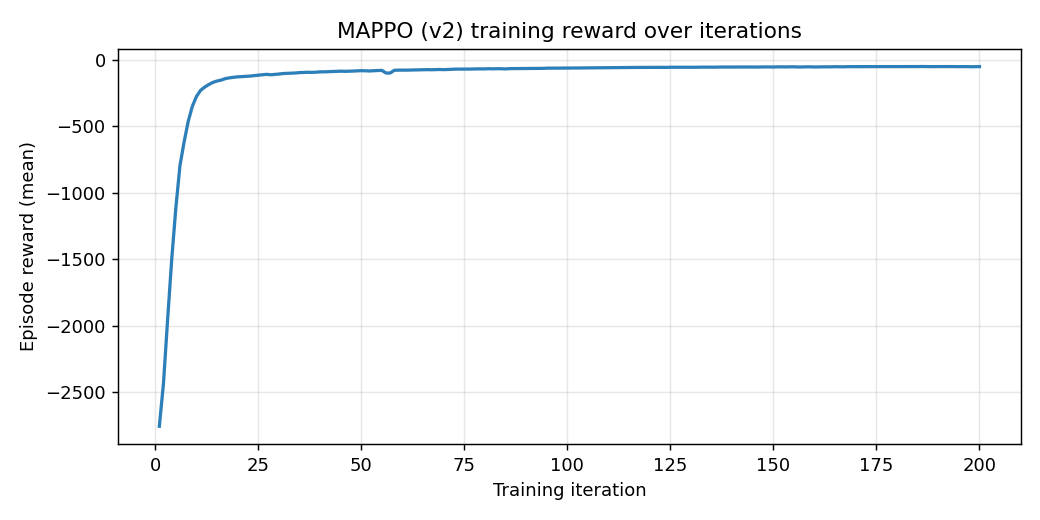
\includegraphics[width=0.7\linewidth]{train_reward.png}
\caption{MAPPO~(v2) mean episode reward over training iterations. Reward rises from
$\approx -2757$ to a stable plateau near $-50$ within roughly 100 iterations.}
\label{fig:trainreward}
\end{figure}

\begin{figure}[H]
\centering
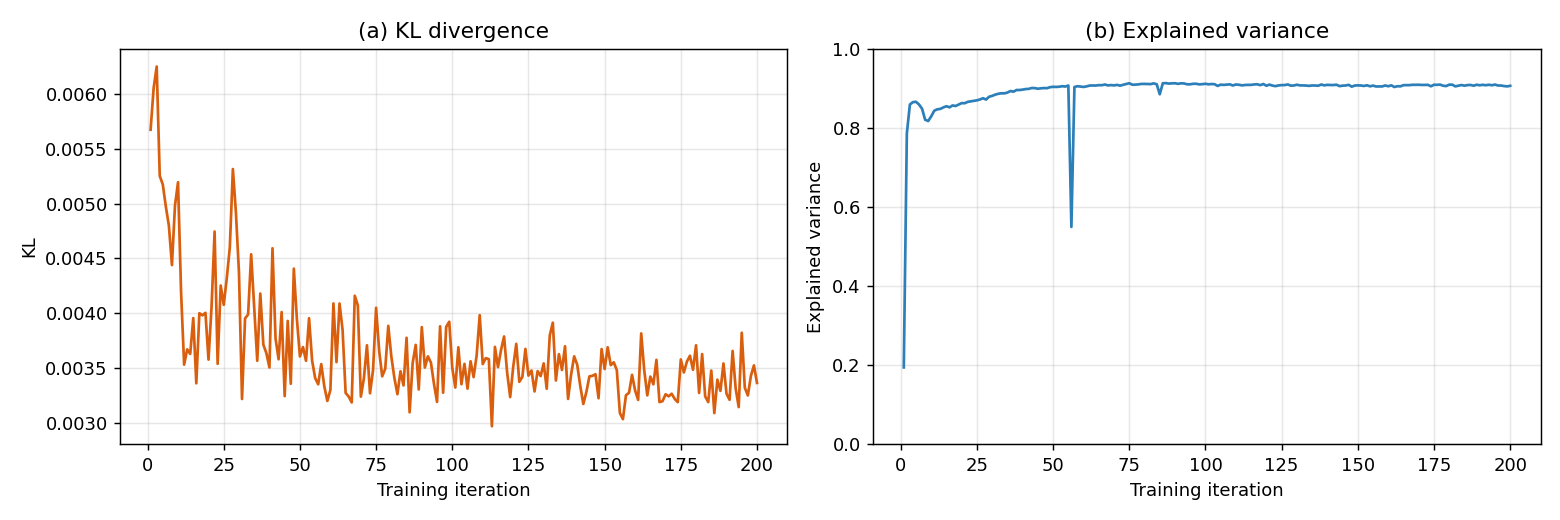
\includegraphics[width=0.92\linewidth]{train_kl_explvar.png}
\caption{Training stability. (a) KL divergence stays small, confirming PPO clipping
constrains the updates. (b) The centralized critic's explained variance climbs to
$\approx 0.91$, indicating accurate value prediction.}
\label{fig:trainkl}
\end{figure}

\section{Comparison Against Heuristic Baselines (Fair Clearance)}
\label{sec:baselines}
A subtle but decisive evaluation issue must be addressed first. The learned agents
pay a \SI{3}{\second} all-red safety clearance on every phase change, whereas the
heuristic controllers, by default, switched instantaneously. Evaluated under that
\emph{unfair} zero-clearance setting, max-pressure appears competitive
($8.15 \pm 0.08$~s average wait). But when the \emph{same} \SI{3}{\second} clearance
is applied to the heuristics --- the cost the learned agents always paid ---
max-pressure's average wait nearly triples to $21.63 \pm 1.00$~s and fixed-time rises
to $47.03 \pm 0.59$~s (Table~\ref{tab:fair}, Figure~\ref{fig:fair}). Under this fair,
matched-clearance protocol the MAPPO controller ($9.92 \pm 0.65$~s) outperforms
max-pressure by roughly a factor of two and fixed-time by nearly a factor of five.
The heuristics' apparent strength was therefore an artefact of an unequal evaluation,
not a genuine advantage; correcting it both restores a fair comparison and
strengthens the case for the learned controllers.

\begin{table}[H]
\centering
\caption{Average waiting time (s) by controller, with and without the
\SI{3}{\second} safety clearance (mean~$\pm$~std over seeds 42--46). The learned
controllers were always evaluated at \SI{3}{\second}; only the matched-clearance
column is a fair comparison.}
\label{tab:fair}
\small
\begin{tabular}{@{}lcc@{}}
\toprule
\textbf{Controller} & \textbf{0\,s clearance (unfair)} & \textbf{3\,s clearance (fair)} \\
\midrule
MAPPO (v2)    & ---            & $\mathbf{9.92 \pm 0.65}$ \\
IPPO          & ---            & $10.34 \pm 0.31$ \\
Max-Pressure  & $8.15 \pm 0.08$ & $21.63 \pm 1.00$ \\
Fixed-Time    & $38.02 \pm 0.81$ & $47.03 \pm 0.59$ \\
\bottomrule
\end{tabular}
\end{table}

\begin{figure}[H]
\centering

\includegraphics[width=\linewidth]{fair_comparison.png}
\caption{Left: average waiting time for all controllers under matched
\SI{3}{\second} clearance --- the learned controllers clearly win. Right: the
confound --- charging the heuristics the same clearance they had been spared erases
their apparent edge, lifting them well above the learned-controller band (shaded).}
\label{fig:fair}
\end{figure}

\section{Fidelity Check Against the Published Recipe}
To rule out the possibility that the cooperative controller is an under-powered
strawman, it is compared against the canonical MAPPO recipe of
Yu~et~al.~\cite{yu2021mappo} ($512 \times 512$ networks; see
Chapter~\ref{ch:methodology}). The two are statistically indistinguishable on
average wait ($9.92 \pm 0.65$~s for the project's MAPPO versus $10.21 \pm 0.28$~s for
the paper recipe; Welch's $t$-test $p = 0.39$), with the project's configuration
numerically slightly ahead. The implemented MAPPO is therefore a faithful and
competitive representative of the method --- which makes the comparison that follows
meaningful: any failure to beat independent learners cannot be blamed on a weak
MAPPO.

\section{The Central Result: Coordination Value \texorpdfstring{$\approx 0$}{= 0}}
\label{sec:twist}
MAPPO is the sophisticated, theoretically motivated choice, with a centralized critic
designed to tame non-stationarity and solve credit assignment and a neighbour-coupled
reward that explicitly encodes coordination. One expects it to beat a set of
independent learners that ignore all of this. It does not.

Against IPPO --- identical in every respect except its decentralized critic and its
purely local reward --- MAPPO is \emph{statistically indistinguishable on every
traffic-performance metric} across five seeds (Table~\ref{tab:coord},
Figure~\ref{fig:coord}): average waiting time ($p = 0.24$), average halting
($p = 0.53$), maximum halting ($p = 0.74$), and completed trips ($p = 0.55$) all show
no significant difference. The \emph{only} reliable difference is that MAPPO performs
about 21 more phase switches per episode ($1391 \pm 12$ versus $1369.6 \pm 8.4$,
$p = 0.015$) --- additional control activity that yields no measurable performance
benefit. The coordination value, defined as $\text{MAPPO} - \text{IPPO}$, is thus
approximately zero on this network.

\begin{table}[H]
\centering
\caption{MAPPO versus IPPO across all evaluation metrics (mean~$\pm$~std over seeds
42--46; $p$ from Welch's $t$-test). Only the phase-switch count differs
significantly, and it favours neither controller in performance terms.}
\label{tab:coord}
\small
\begin{tabular}{@{}lccc@{}}
\toprule
\textbf{Metric} & \textbf{MAPPO} & \textbf{IPPO} & \textbf{$p$-value} \\
\midrule
Average wait (s)     & $9.92 \pm 0.65$   & $10.34 \pm 0.31$  & $0.236$ \\
Average halting      & $3.91 \pm 0.11$   & $4.00 \pm 0.27$   & $0.534$ \\
Maximum halting      & $14.2 \pm 1.6$    & $14.6 \pm 2.1$    & $0.745$ \\
Completed trips      & $1261.6 \pm 0.9$  & $1261.2 \pm 1.1$  & $0.545$ \\
Phase switches       & $1391 \pm 12$     & $1370 \pm 8$      & $\mathbf{0.015}$ \\
\bottomrule
\end{tabular}
\end{table}

\begin{figure}[H]
\centering
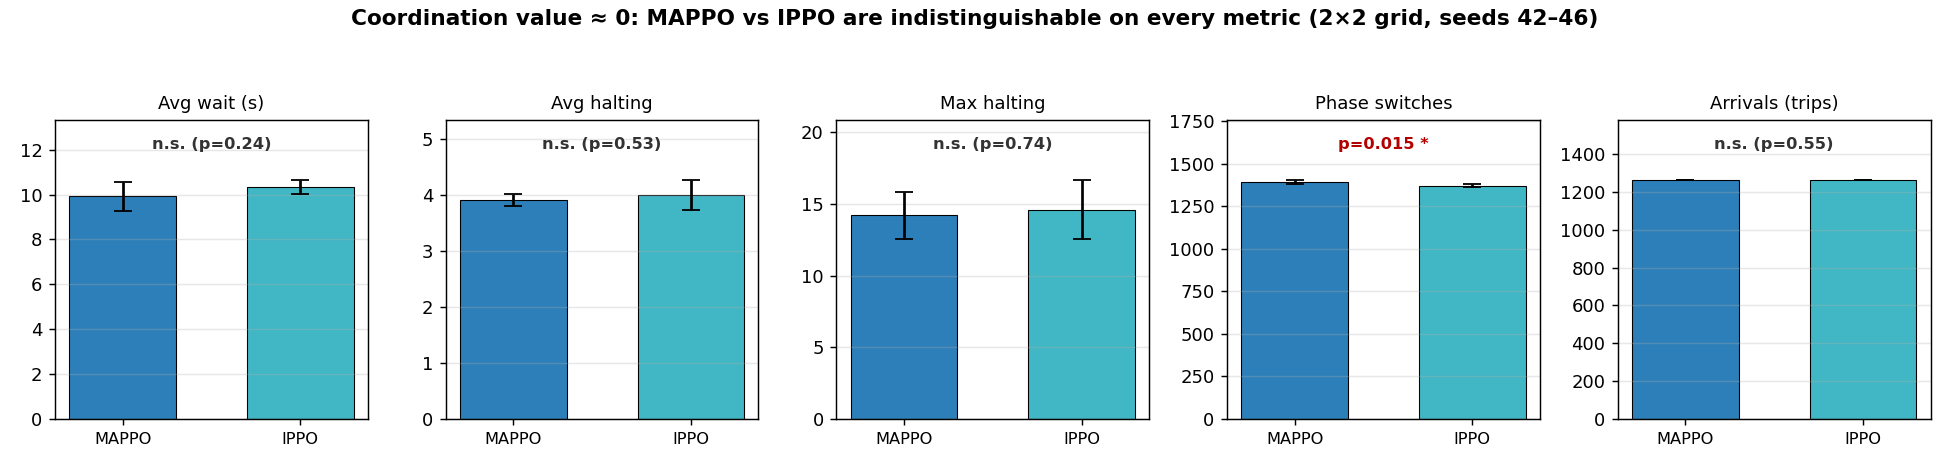
\includegraphics[width=\linewidth]{coordination_value.png}
\caption{The central finding. Across all five metrics, MAPPO and IPPO are
statistically indistinguishable (``n.s.''), except for a small, performance-neutral
difference in phase-switch count. The explicit coordination machinery buys no
measurable advantage on the $2\times2$ network.}
\label{fig:coord}
\end{figure}

\noindent This is the plot twist the dissertation set out to surface: on a small,
inherently cooperative network, the full cooperative MARL package performs no better
than independent learners. Chapter~\ref{ch:discussion} examines why, and
Chapter~\ref{ch:futurework} sets out the experiments that would test the resulting
hypothesis.

\chapter{Discussion}
\label{ch:discussion}

The results of Chapter~\ref{ch:results} invert the expectation that frames most of
the cooperative-MARL literature. MAPPO is the sophisticated, theoretically motivated
choice: its centralized critic is designed precisely to tame non-stationarity and to
solve the multi-agent credit-assignment problem, and its neighbour-coupled reward
explicitly encodes coordination. One naturally expects it to beat a set of
independent learners that ignore all of this. Yet on the \grid{2} network the two
are statistically indistinguishable on every performance metric, and the only
reliable difference --- MAPPO's slightly higher switching rate --- is, if anything, a
mild inefficiency rather than a benefit. This chapter asks why.

\section{Why the Coordination Value Is Near Zero}
The most parsimonious explanation is that, at this scale, \emph{there is little
coordination left for an explicit mechanism to add}. A \grid{2} grid has only four
intersections, each adjacent to two neighbours, and the traffic-control reward is
already locally informative: minimizing one's own queue and waiting time, on a
network this tightly coupled, is almost the same objective as minimizing the
network's. In other words, the incentives are \emph{already aligned} by the
structure of the problem. The centralized critic provides a lower-variance value
estimate and the neighbour-pressure term nudges toward network-aware behaviour, but
an independent learner equipped with the same local observations and the same
parameter-sharing can discover the same coordinated phasing on its own. Coordination
here is \emph{emergent} rather than \emph{engineered}: it falls out of independent
optimization because the environment does not reward defection.

This reading is reinforced by two details. First, both learned controllers
\emph{decisively} beat the heuristic baselines under matched clearance
(Chapter~\ref{ch:results}); the learning is doing real work --- it is not that the
task is trivial, but that the \emph{coordination-specific} additions are redundant.
Second, MAPPO's extra phase switches buy no improvement, which is consistent with a
centralized critic that is active but not pivotal: it shapes the policy slightly
differently without changing what the policy ultimately achieves.

\section{The Scale Hypothesis}
If the coordination value is small \emph{because} the network is small, then it
should grow with scale. As a grid enlarges, an agent's actions influence ever more
distant intersections through longer chains of traffic; the gap between ``minimize
my own delay'' and ``minimize the network's delay'' widens, non-stationarity from
the perspective of any single learner intensifies, and the centralized critic's
access to the global state should translate into a measurable advantage. This is
exactly the regime in which network-level cooperation has been shown to
matter: CoLight~\cite{wei2019colight} demonstrates gains from sharing neighbour
information at city scale, and the large-scale study of
Chu~et~al.~\cite{chu2020largescale} reports that neighbour-aware, carefully designed
shared rewards improve performance --- while naive individual rewards can actively
harm throughput --- on large networks. The near-zero coordination value measured here
is therefore not in tension with that literature; it is the expected
\emph{small-scale} end of the same curve.

\section{Implications}
The practical implication is a note of caution and a research direction. The caution
is that, on small or tightly coupled multi-agent problems, the considerable
machinery of CTDE may be unnecessary: a simpler independent-learning approach with
parameter sharing can match it, at lower implementation and training cost. The
research direction is that the \emph{value of coordination} should be treated as a
quantity that depends on system scale and on how strongly incentives conflict ---
not as a fixed property of an algorithm. The controlled traffic setting used here
establishes a clean zero-point for that quantity, against which both larger networks
and genuine social dilemmas (Chapter~\ref{ch:futurework}) can be measured.

\chapter{Future Work}
\label{ch:futurework}

The central finding of this dissertation --- that an explicit coordination mechanism
buys essentially nothing over independent learners on a \grid{2} traffic network ---
is best read not as an endpoint but as a precisely located starting point. Two
directions follow directly, both placed beyond the scope of this submission by
compute constraints rather than by design.

\section{Network Scale-Up (\texorpdfstring{\grid{2} $\rightarrow$ \grid{5}}{2x2 to 5x5})}
The most direct test of the interpretation in Chapter~\ref{ch:discussion} is to
grow the network. If the coordination value is near zero because a \grid{2} grid is
small enough that incentives are already locally aligned, then enlarging the network
to \grid{5} (25 intersections) should widen the gap between MAPPO and IPPO: distant
intersections interact through longer traffic chains, non-stationarity intensifies,
and the centralized critic's global view should begin to pay off. This expectation
is consistent with the large-scale findings of Chu~et~al.~\cite{chu2020largescale}
and the network-level cooperation of CoLight~\cite{wei2019colight}. A \grid{5} SUMO
network skeleton was prototyped during this project but reverted; training it to
convergence at this scale (with a single GPU and per-run training times measured in
days) exceeded the available compute budget. Quantifying how coordination value
scales with network size is therefore the primary item of future work.

\section{Extending to a Social Dilemma}
Traffic occupies the pure-coordination end of the cooperation spectrum: incentives
are aligned, so there is nothing to defect over. The complementary experiment is to
move to the \emph{opposite} end --- a sequential social dilemma in which defection is
individually tempting but collectively harmful. A natural choice is an
apple-harvesting commons in the style of Leibo~et~al.~\cite{leibo2017ssd}, where
agents collect a slowly regrowing resource and over-harvesting permanently depletes
it. There, the reward-structure axis (individual versus shared rewards) that is
inert in traffic should become decisive, allowing a direct study of when shared
rewards are \emph{necessary} to sustain cooperation versus when independent learning
suffices. Contrasting the learned behaviours across the two environments would
complete the coordination--dilemma spectrum this project set out to chart.

\section{Efficiency--Equity Analysis}
Finally, the per-agent breakdowns collected here can support a fairness analysis
(e.g.\ a Gini coefficient over per-intersection outcomes) to determine whether high
system performance requires unequal treatment of individual intersections --- a
question that becomes more pointed at larger scales and in dilemma settings.

\chapter{Conclusion}
\label{ch:conclusion}

This dissertation set out to test a simple but consequential question on a
controlled traffic benchmark: does an explicitly cooperative multi-agent algorithm
actually outperform a set of independent learners when the two are matched in every
other respect? The investigation produced a clear, and initially surprising, answer.

A MAPPO traffic-signal controller was implemented on a \grid{2} grid, trained to
stable convergence, and shown --- under a \emph{fair}, matched-clearance evaluation ---
to outperform both the fixed-time and max-pressure heuristics decisively. A
methodological contribution emerged along the way: the heuristic baselines had been
flattered by an unfair zero-clearance evaluation, and correcting it (charging every
controller the same safety clearance) both restored a fair comparison and
strengthened the case for the learned controllers. The project's MAPPO was further
confirmed to be a faithful implementation by matching the canonical published
recipe.

The central result is that, against this strong and faithful MAPPO, an Independent
PPO comparator --- differing only in its decentralized critic and purely local
reward --- proved \emph{statistically indistinguishable} on every traffic-performance
metric. The sophisticated coordination machinery bought no measurable advantage; its
only distinguishing behaviour was a slightly higher rate of phase switching that
produced no benefit. On a \grid{2} network, the \emph{coordination value} is
approximately zero.

The interpretation is not that coordination is worthless, but that the testbed is
too small to require it: at this scale incentives are already locally aligned, and
independent learners recover coordinated behaviour implicitly. This precisely
locates where explicit coordination should begin to matter --- at larger network
scales --- and motivates the future work of scaling to \grid{5} and of extending the
study to genuine social dilemmas, where reward structure and the temptation to
defect are expected to make coordination indispensable. The contribution of this
work is thus both a careful negative result and a sharpened hypothesis: the value of
cooperation in multi-agent reinforcement learning is not a constant but a function
of scale, and the controlled traffic setting establishes the baseline against which
that function can now be measured.


% ----------------------------- REFERENCES -----------------------------
\bibliographystyle{IEEEtran}
\bibliography{references}

\end{document}
